
\textcolor{red}{Falta definicion de distancia, de norma y la relacion entre ellas.  Como ejemplo poner la norma 1 y 2. Graficar algunos mismos conjuntos con diferente normas}



\begin{definition} [Bola de radio $\delta$ y centro $x_o$] \label{def:bola}
    Sean $x_o \in \Rn{n},\;\delta > 0$ y $\text{d}$ una distancia en $\Rn{n}$. La \emph{bola de radio $\delta$ y centro $x_o$}, que denotamos con $B_{\delta}(x_o)$, es el conjunto:
    \[
     B_{\delta}(x_o) = \left\lbrace x \in \Rn{n} : \text{d}(x,x_o) < \delta \right\rbrace.
    \]
    El conjunto
    \[
     B^*_{\delta}(x_o) = B_{\delta}(x_o) - \{ x_o \}
    \]
    es la \emph{bola reducida de radio $\delta$ y centro $x_o$}.
   
   \end{definition}
   
   \begin{definition} [Punto interior, interior de un conjunto] \label{def:interior}
    Sean $A \subset \Rn{n} \text{ y } x_o \in A$. Decimos que $x_o$ es \emph{punto interior} de $A$ si
    \[
     \exists \delta > 0 / B_{\delta}(x_o) \subset A.
    \]
    El \emph{interior} de $A$, que denotamos con $A^{\circ}$, es el conjunto de todos los puntos interiores de $A$:
    \[
    A^{\circ}= \left\lbrace x \in A : x \text{ es punto interior de } A \right\rbrace.
    \]
   \end{definition}
   
   
   \begin{definition} [Conjunto abierto] \label{def:abierto}
       Sea $A \subset \Rn{n}$. Decimos que $A$ es \emph{abierto} si
   \[
        \forall x_o \in \exists \delta > 0 : B_{\delta}(x_o) \subset A.\footnote{\text{i.e.: $A$  es abierto si todos sus puntos son interiores.}}
   \]
   \end{definition}
   
   \begin{propertie}  \label{prop:abierto_int}    Sea  $A \subseteq \Rn{n}$
   
    1.  $A \subseteq  A^{\circ}.$      \:\:\:\:\:\:\:\:\:\:\:\:\:\:\:\:\:\:\:\:                        2.  $\text{   A  es abierto }  \iff   A =  A^{\circ}.$
    \end{propertie}
   
   \begin{definition} [Conjunto cerrado] \label{def:cerrado}
    Sea $A \subset \Rn{n}$. Decimos que $A$ es \emph{cerrado} si su complemento $A^c = \Rn{n} - A$ es abierto.
   \end{definition}
   
   \begin{definition} [Frontera de un conjunto] \label{def:frontera}
    Sea $A \subset \Rn{n}$. La \emph{frontera} de $A$, que denotamos con $\front A$ o $\frontera(A)$, es el conjunto:
    \[
     \front A = \left\lbrace x_o \in \Rn{n} : \forall \delta > 0 \,
     B_{\delta}(x_o) \cap A \ne \emptyset \wedge
     B_{\delta}(x_o) \cap A^c \ne \emptyset \right\rbrace.
    \]
   \end{definition}
   
   \begin{propertie} \label{prop:cerrado_front}
    Un conjunto $A \subset \Rn{n}$ es cerrado si y solo si $\front A \subset A$.
   \end{propertie}
   
   \begin{definition} [Punto de acumulaci\'on] \label{def:pto_acum}
    Sean $A \subset \Rn{n} \text{ y } x_o \in \Rn{n}$. Decimos que $x_o$ es \emph{punto de acumulaci\'on} de $A$ si
    \[
     \forall \delta > 0 \left( B_{\delta}(x_o) - \{ x_o \} \right) \cap A \ne \emptyset. 
    \]
    Denotamos el conjunto de todos los puntos de acumulaci\'on de $A$ con $A'$:
    \[
     A' = \{ x \in \Rn{n} : x \text{ es punto de acumulaci\'on de } A \}.
    \]
   
   \end{definition}
   
   \begin{definition} [Entorno de un punto] \label{def:entorno}
    Sean $N \subset  \Rn{n}$ y $x_o \in \Rn{n}$. Decimos que $N$ es \emph{entorno} de $x_o$ si
    \[
     \exists \delta > 0 : B_{\delta}(x_o) \subset N.
    \]
   \end{definition}
   
   \begin{definition} [Punto aislado] \label{def:pto_ais}
    Sean $A \subset  \Rn{n}$ y $x_o \in A$. Decimos que $x_o$ es \emph{punto aislado} de $A$ si $x_o$ no es punto de acumulaci\'on de $A$.
   \end{definition}
   
   \begin{definition} [Conjunto acotado] \label{def:conj_acotado}
    Sea $A \subset \Rn{n}$. Decimos que $A$ es un \emph{conjunto acotado} si existe $\delta > 0$ tal que la bola de radio $\delta$  centrada en el origen contiene al conjunto $A$, es decir, si $\exists \delta > 0 : A \subset B_{\delta}(\mathbf{0})$.\\
    Equivalentemente, $A$ es un \emph{conjunto acotado} si $\exists \delta > 0, x_o \in \Rn{n} : A \subset B_{\delta}(x_o)$.
   \end{definition}
   
   
   \begin{definition}
    Sea un conjunto $A\subseteq\Rn{n}$. $A$ se llama \textbf{conexo} si dados dos puntos cualquiera de $A$ se los puede unir por una curva continua que este incluida en $A$.
\end{definition}
   
   


%------------------------------------------------------conjunto conexo----------------------------
\begin{definition} [Conjunto conexo] \label{def:conjuntoconexo} Un conjunto \( A \subset \mathbb{R}^n \) es \textbf{conexo} si para cualesquiera dos puntos \( x_0, y_0 \in A \), existe una curva continua \( \gamma : [0,1] \to A \) tal que:

    \[
    \gamma(0) = x_1 \quad \text{y} \quad \gamma(1) = y_1
    \]
    
    
    \begin{center}
        \begin{minipage}{0.45\textwidth}
            \centering
            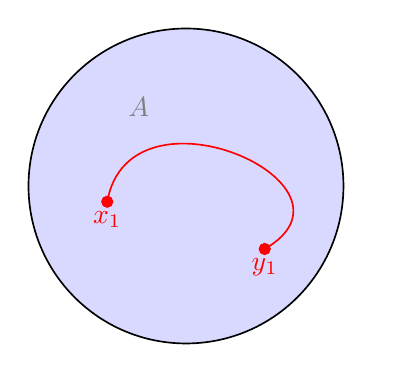
\begin{tikzpicture}
                \draw[fill=blue!15, semithick] (0,0) circle(2);
                \filldraw[red] (-1,-0.2) circle (2pt) node[below] {\(x_1\)};
                \filldraw[red] (1,-0.8) circle (2pt) node[below] {\(y_1\)};
                \draw[semithick,-,red] (-1,-0.2) to[out=80,in=30,looseness=2] (1,-0.8);
                \draw node at (-0.6,1) {\textcolor{gray}{$A$}};
            \end{tikzpicture}
        \end{minipage}
        \hspace{1cm} % espacio entre figuras
        \begin{minipage}{0.45\textwidth}
            \centering
            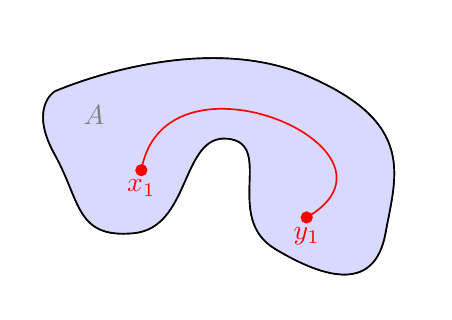
\begin{tikzpicture}
       
                % Plane R^2 on the right
               
                    \draw[semithick]
                        plot[smooth,tension=1.2] coordinates {(-0.2,0.8) (3,1) (4,-1) (2.6,-1.2)(2,0.2) (0.8,-1) (-0.2,0)(-0.2,0.8)};
                    
                    \filldraw[fill=blue!15, semithick]
                        plot[smooth, tension=1.2] coordinates {(-0.2,0.8) (3,1) (4,-1) (2.6,-1.2)(2,0.2) (0.8,-1) (-0.2,0)(-0.2,0.8)};
                        % \foreach \point in {(1,0.6), (3,0), (2.5,-1.5), (1,-1), (0.2,0.1), (1,0.6)} {
                        % \node at \point [circle,fill,inner sep=1pt] {};
                        % }
                    \filldraw[red] (0.9,-0.2) circle (2pt) node[below] {\(x_1\)};
                    \filldraw[red] (3,-0.8) circle (2pt) node[below] {\(y_1\)};
                    \draw[semithick,-,red] (0.9,-0.2) to[out=80,in=30,looseness=2] (3,-0.8);
                    \draw node at (0.3,0.5) {\textcolor{gray}{$A$}};
                    
            
            \end{tikzpicture}
        \end{minipage}
        \end{center}
        \begin{center}
        
\begin{tikzpicture}
            \node at (1.5,-2) {Conjuntos \textbf{conexos}};
        \end{tikzpicture}
        \end{center}
    \end{definition}
    
    %------------------------------------------------------conjunto conexo----------------------------
    \begin{definition} [Conjunto convexo] \label{def:conjuntoconvexo}Un subconjunto \( A \subseteq \mathbb{R}^n \) es \textbf{convexo} si para cualesquiera dos puntos \( x, y \in A \), el segmento que los une está completamente contenido en \( A \):
        \[
        \forall x_1,y_1, \quad \lambda x + (1 - \lambda)y \in A \quad \text{para todo } \lambda \in [0,1].
        \]
        
    
    
    
    
        \begin{center}
            \begin{minipage}{0.45\textwidth}
                \centering
                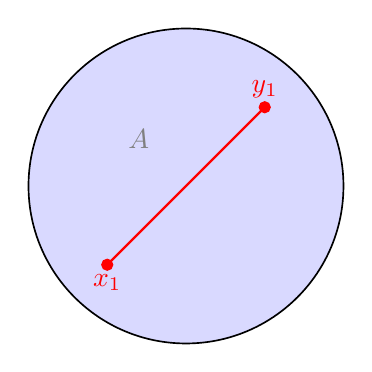
\begin{tikzpicture}
                    \draw[fill=blue!15, semithick] (0,0) circle(2);
                    \filldraw[red] (-1,-1) circle (2pt) node[below] {\(x_1\)};
                    \filldraw[red] (1,1) circle (2pt) node[above] {\(y_1\)};
                    \draw[thick, red, domain=-1:1] plot (\x, {\x});
                    \draw node at (-0.6,0.6) {\textcolor{gray}{$A$}};
                \end{tikzpicture}
            \end{minipage}
            \hspace{1cm} % espacio entre figuras
            \begin{minipage}{0.45\textwidth}
                \centering
                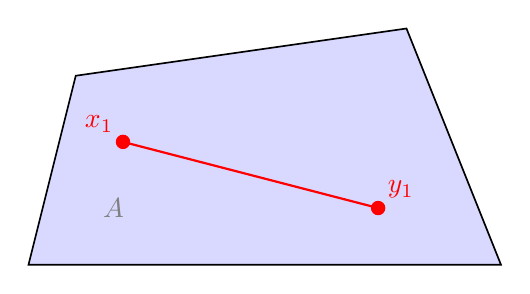
\begin{tikzpicture}[scale=1.2]
                    \filldraw[fill=blue!15, semithick] (-1.5,0) -- (3.5,0) -- (2.5,2.5) -- (-1,2) -- cycle;
                    \draw[thick, red] (-0.5,1.3) -- (2.2,0.6);
                    \filldraw[red] (-0.5,1.3) circle (2pt) node[above left] {\(x_1\)};
                    \filldraw[red] (2.2,0.6) circle (2pt) node[above right] {\(y_1\)};
                    \draw node at (-0.6,0.6) {\textcolor{gray}{$A$}};
                \end{tikzpicture}
            \end{minipage}
            \end{center}
            \begin{center}
            
\begin{tikzpicture}
                \node at (1.5,-2) {Conjuntos \textbf{convexos}};
            \end{tikzpicture}
    
            \end{center}
            \begin{center}
                \begin{minipage}{0.45\textwidth}
                    \centering
                    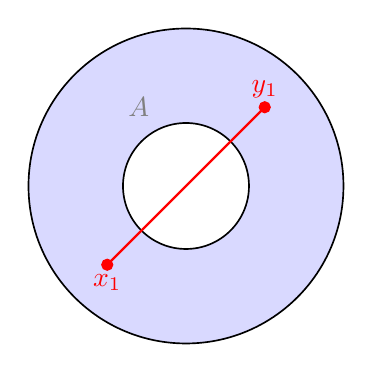
\begin{tikzpicture}
                        % Círculo exterior (azul claro) \draw[fill=blue!15, semithick] (0,0) circle(2);
                        \draw[fill=blue!15, semithick] (0,0) circle(2);
                        
                        % Círculo interior (blanco, para el hueco)
                        \draw[fill=white, semithick] (0,0) circle(0.8);
                        
                        \filldraw[red] (-1,-1) circle (2pt) node[below] {\(x_1\)};
                        \filldraw[red] (1,1) circle (2pt) node[above] {\(y_1\)};
                        \draw[thick, red, domain=-1:1] plot (\x, {\x});
                        
                        % Letra A
                        \draw node at (-0.6,1) {\textcolor{gray}{$A$}};
                    \end{tikzpicture}
                \end{minipage}
                \hspace{1cm} % espacio entre figuras
                \begin{minipage}{0.45\textwidth}
                    \centering
                    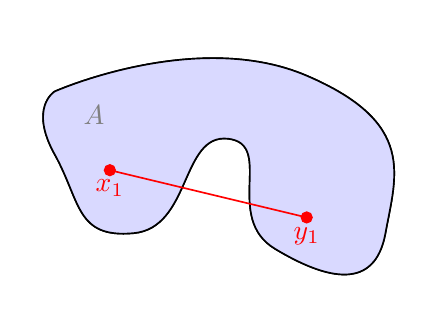
\begin{tikzpicture}
               
                        % Plane R^2 on the right
                       
                            \draw[semithick]
                                plot[smooth,tension=1.2] coordinates {(-0.2,0.8) (3,1) (4,-1) (2.6,-1.2)(2,0.2) (0.8,-1) (-0.2,0)(-0.2,0.8)};
                            
                            \filldraw[fill=blue!15, semithick]
                                plot[smooth, tension=1.2] coordinates {(-0.2,0.8) (3,1) (4,-1) (2.6,-1.2)(2,0.2) (0.8,-1) (-0.2,0)(-0.2,0.8)};
                                % \foreach \point in {(1,0.6), (3,0), (2.5,-1.5), (1,-1), (0.2,0.1), (1,0.6)} {
                                % \node at \point [circle,fill,inner sep=1pt] {};
                                % }
                                \filldraw[red] (0.5,-0.2) circle (2pt) node[below] {\(x_1\)};
                                \filldraw[red] (3,-0.8) circle (2pt) node[below] {\(y_1\)};
                                \draw[semithick, red] (0.5,-0.2) -- (3,-0.8); % Línea recta
                            \draw node at (0.3,0.5) {\textcolor{gray}{$A$}};
                            
                    
                    \end{tikzpicture}
                \end{minipage}
                \end{center}
                \begin{center}
                
\begin{tikzpicture}
                    \node at (1.5,-2) {Conjuntos \textbf{NO convexos}};
                \end{tikzpicture}
                \end{center}
    \end{definition}
    
    %------------------------------------------------------conjunto simplemente conexo----------------------------
    \vspace{0.5cm}
    \begin{definition}[Conjunto conexo] \label{def:conjuntoconexo}
    Un conjunto \( A \subset \mathbb{R}^2 \) es \textbf{simplemente conexo} si es conexo y todo lazo cerrado dentro de \( A \) puede ser continuamente deformado a un punto, sin salir de \( A \).
    
    \vspace{0.3cm} % Pequeño espacio entre el texto y las figuras
    
    \begin{center}
        \begin{minipage}{0.45\textwidth}
            \centering
            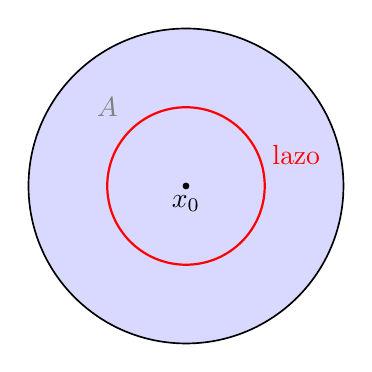
\begin{tikzpicture}
                \draw[fill=blue!15, semithick] (0,0) circle(2);
                \draw[red, thick] (0,0) circle(1);
                \node at (-1,1) {\textcolor{gray}{$A$}};
                \node at (1.4,0.4) {\textcolor{red}{lazo}};
                \filldraw[black] (0,0) circle (1pt) node[below] {\(x_0\)};
            \end{tikzpicture}
        \end{minipage}
        \hspace{1cm}
        \begin{minipage}{0.45\textwidth}
            \centering
            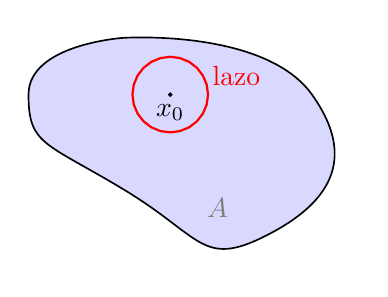
\begin{tikzpicture}[scale=1.2]
                \filldraw[fill=blue!15, semithick]
                    plot[smooth, tension=1.2] coordinates {(1,0.6) (3,0) (2.5,-1.5) (1,-1) (0,0) (1,0.6)};
                \draw[thick, red, domain=0:360] plot ({1.5 + 0.4*cos(\x)}, {0 + 0.4*sin(\x)});
                \node at (2,-1.2) {\textcolor{gray}{$A$}};
                \node[red] at (2.2,0.2) {lazo};
                \filldraw[black] (1.5,0) circle (0.5pt) node[below] {\(x_0\)};
            \end{tikzpicture}
        \end{minipage}
    \end{center}
    
    \vspace{0.3cm} % Pequeño espacio antes de la etiqueta
    
    \begin{center}
        
\begin{tikzpicture}
            \node at (1.5,-2) {Conjuntos \textbf{simplemente conexos}};
        \end{tikzpicture}
    \end{center}
    
    \begin{center}
        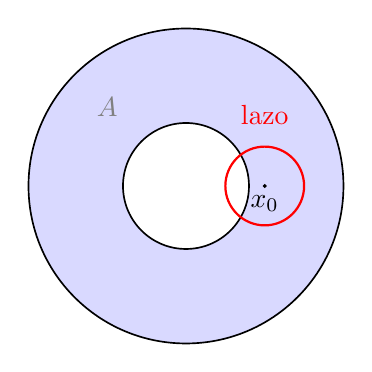
\begin{tikzpicture}
            % Círculo exterior (azul claro) \draw[fill=blue!15, semithick] (0,0) circle(2);
            \draw[fill=blue!15, semithick] (0,0) circle(2);
            
            % Círculo interior (blanco, para el hueco)
            \draw[fill=white, semithick] (0,0) circle(0.8);
            
            \draw[red, thick] (1,0) circle(0.5);
                \node at (-1,1) {\textcolor{gray}{$A$}};
                \node at (1,0.9) {\textcolor{red}{lazo}};
                \filldraw[black] (1,0) circle (0.5pt) node[below] {\(x_0\)};
        \end{tikzpicture}
        \end{center}
        \begin{center}
            
\begin{tikzpicture}
                \node at (1.5,-2) {Conjunto \textbf{NO simplemente conexo}};
            \end{tikzpicture}
        \end{center}
    \end{definition}
    
    
    
    
    
    
    
    
    
    
    
   
   
   